\documentclass[a4paper]{book}
\usepackage{a4wide}
\usepackage{makeidx}
\usepackage{graphicx}
\usepackage{multicol}
\usepackage{float}
\usepackage{listings}
\usepackage{color}
\usepackage{textcomp}
\usepackage{alltt}
\usepackage{times}
\usepackage{ifpdf}
\ifpdf
\usepackage[pdftex,
            pagebackref=true,
            colorlinks=true,
            linkcolor=blue,
            unicode
           ]{hyperref}
\else
\usepackage[ps2pdf,
            pagebackref=true,
            colorlinks=true,
            linkcolor=blue,
            unicode
           ]{hyperref}
\usepackage{pspicture}
\fi
\usepackage[utf8]{inputenc}
\usepackage{doxygen}
\lstset{language=C++,inputencoding=utf8,basicstyle=\footnotesize,breaklines=true,breakatwhitespace=true,tabsize=8,numbers=left }
\makeindex
\setcounter{tocdepth}{3}
\renewcommand{\footrulewidth}{0.4pt}
\begin{document}
\hypersetup{pageanchor=false}
\begin{titlepage}
\vspace*{7cm}
\begin{center}
{\Large OpenKIMTests \\[1ex]\large 0.1 }\\
\vspace*{1cm}
{\large Generated by Doxygen 1.7.1}\\
\vspace*{0.5cm}
{\small Wed Feb 2 2011 21:35:05}\\
\end{center}
\end{titlepage}
\clearemptydoublepage
\pagenumbering{roman}
\tableofcontents
\clearemptydoublepage
\pagenumbering{arabic}
\hypersetup{pageanchor=true}
\chapter{Class Index}
\section{Class Hierarchy}
This inheritance list is sorted roughly, but not completely, alphabetically:\begin{DoxyCompactList}
\item \contentsline{section}{BaseTest::BaseTest}{\pageref{classBaseTest_1_1BaseTest}}{}
\begin{DoxyCompactList}
\item \contentsline{section}{BCCLattice::BCCLattice}{\pageref{classBCCLattice_1_1BCCLattice}}{}
\item \contentsline{section}{ElasticModulus::ElasticModulus}{\pageref{classElasticModulus_1_1ElasticModulus}}{}
\item \contentsline{section}{FCCLattice::FCCLattice}{\pageref{classFCCLattice_1_1FCCLattice}}{}
\item \contentsline{section}{NullTest::NullTest}{\pageref{classNullTest_1_1NullTest}}{}
\end{DoxyCompactList}
\end{DoxyCompactList}

\chapter{Class Index}
\section{Class List}
Here are the classes, structs, unions and interfaces with brief descriptions:\begin{DoxyCompactList}
\item\contentsline{section}{\hyperlink{classBaseTest_1_1BaseTest}{BaseTest::BaseTest} }{\pageref{classBaseTest_1_1BaseTest}}{}
\item\contentsline{section}{\hyperlink{classFCCLattice_1_1FCCLattice}{FCCLattice::FCCLattice} }{\pageref{classFCCLattice_1_1FCCLattice}}{}
\item\contentsline{section}{\hyperlink{classNullTest_1_1NullTest}{NullTest::NullTest} }{\pageref{classNullTest_1_1NullTest}}{}
\end{DoxyCompactList}

\chapter{Class Documentation}
\hypertarget{classBaseTest_1_1BaseTest}{
\section{BaseTest::BaseTest Class Reference}
\label{classBaseTest_1_1BaseTest}\index{BaseTest::BaseTest@{BaseTest::BaseTest}}
}
Inheritance diagram for BaseTest::BaseTest:\begin{figure}[H]
\begin{center}
\leavevmode
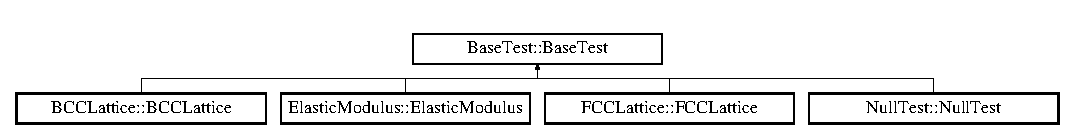
\includegraphics[height=2.000000cm]{classBaseTest_1_1BaseTest}
\end{center}
\end{figure}
\subsection*{Public Member Functions}
\begin{DoxyCompactItemize}
\item 
\hypertarget{classBaseTest_1_1BaseTest_a217c24e20c2abe8be4647faebac3e6ac}{
def {\bfseries \_\-\_\-init\_\-\_\-}}
\label{classBaseTest_1_1BaseTest_a217c24e20c2abe8be4647faebac3e6ac}

\item 
def \hyperlink{classBaseTest_1_1BaseTest_a1deedc89d1061da5e3afbd108af06760}{XMLWriter}
\item 
def \hyperlink{classBaseTest_1_1BaseTest_a69587478d3e6af59228e466411efb626}{getASEPotentialByName}
\item 
def \hyperlink{classBaseTest_1_1BaseTest_ad7b3f3b61fcb07c94ae62cb12f060819}{TestResults}
\item 
def \hyperlink{classBaseTest_1_1BaseTest_a1857df472a65cef53372455376136409}{Verify}
\item 
def \hyperlink{classBaseTest_1_1BaseTest_adace34a3904d856f00286217637b9914}{main}
\end{DoxyCompactItemize}
\subsection*{Public Attributes}
\begin{DoxyCompactItemize}
\item 
\hypertarget{classBaseTest_1_1BaseTest_ab7dc01a5da78c687b1e3ef5695c6bb10}{
{\bfseries potentialname}}
\label{classBaseTest_1_1BaseTest_ab7dc01a5da78c687b1e3ef5695c6bb10}

\item 
\hypertarget{classBaseTest_1_1BaseTest_a0ab2e64475afb484074b0effbab3fbc4}{
{\bfseries potential}}
\label{classBaseTest_1_1BaseTest_a0ab2e64475afb484074b0effbab3fbc4}

\item 
\hypertarget{classBaseTest_1_1BaseTest_a8278580db97a9db5498314f3ea38edb9}{
{\bfseries element}}
\label{classBaseTest_1_1BaseTest_a8278580db97a9db5498314f3ea38edb9}

\item 
\hypertarget{classBaseTest_1_1BaseTest_aa4138cfb9b5dd8906a54427626525971}{
{\bfseries verify}}
\label{classBaseTest_1_1BaseTest_aa4138cfb9b5dd8906a54427626525971}

\item 
\hypertarget{classBaseTest_1_1BaseTest_a709baa7891ff3f65b10303b5bf320f88}{
{\bfseries write}}
\label{classBaseTest_1_1BaseTest_a709baa7891ff3f65b10303b5bf320f88}

\item 
\hypertarget{classBaseTest_1_1BaseTest_a9dc99538651adf4352d5e389221aa646}{
{\bfseries TestDependencies}}
\label{classBaseTest_1_1BaseTest_a9dc99538651adf4352d5e389221aa646}

\end{DoxyCompactItemize}


\subsection{Detailed Description}
\begin{DoxyVerb}This is the Base Test from which all other Tests inherit.\end{DoxyVerb}
 

Definition at line 18 of file BaseTest.py.



\subsection{Member Function Documentation}
\hypertarget{classBaseTest_1_1BaseTest_a69587478d3e6af59228e466411efb626}{
\index{BaseTest::BaseTest@{BaseTest::BaseTest}!getASEPotentialByName@{getASEPotentialByName}}
\index{getASEPotentialByName@{getASEPotentialByName}!BaseTest::BaseTest@{BaseTest::BaseTest}}
\subsubsection[{getASEPotentialByName}]{\setlength{\rightskip}{0pt plus 5cm}def BaseTest::BaseTest::getASEPotentialByName (
\begin{DoxyParamCaption}
\item[{}]{ self, }
\item[{}]{ name}
\end{DoxyParamCaption}
)}}
\label{classBaseTest_1_1BaseTest_a69587478d3e6af59228e466411efb626}
\begin{DoxyVerb}A little helper method to call ASE potentials by name. 

In the future, to be extended to include KIM potentials\end{DoxyVerb}
 

Definition at line 96 of file BaseTest.py.

\hypertarget{classBaseTest_1_1BaseTest_adace34a3904d856f00286217637b9914}{
\index{BaseTest::BaseTest@{BaseTest::BaseTest}!main@{main}}
\index{main@{main}!BaseTest::BaseTest@{BaseTest::BaseTest}}
\subsubsection[{main}]{\setlength{\rightskip}{0pt plus 5cm}def BaseTest::BaseTest::main (
\begin{DoxyParamCaption}
\item[{}]{ self}
\end{DoxyParamCaption}
)}}
\label{classBaseTest_1_1BaseTest_adace34a3904d856f00286217637b9914}
\begin{DoxyVerb}Main is called when the Test is run from the command line. currently runs tests
and passes the dictionary of results to the XMLWriter Method\end{DoxyVerb}
 

Definition at line 116 of file BaseTest.py.

\hypertarget{classBaseTest_1_1BaseTest_ad7b3f3b61fcb07c94ae62cb12f060819}{
\index{BaseTest::BaseTest@{BaseTest::BaseTest}!TestResults@{TestResults}}
\index{TestResults@{TestResults}!BaseTest::BaseTest@{BaseTest::BaseTest}}
\subsubsection[{TestResults}]{\setlength{\rightskip}{0pt plus 5cm}def BaseTest::BaseTest::TestResults (
\begin{DoxyParamCaption}
\item[{}]{ self}
\end{DoxyParamCaption}
)}}
\label{classBaseTest_1_1BaseTest_ad7b3f3b61fcb07c94ae62cb12f060819}
\begin{DoxyVerb}The Test Results method, runs the test and packages the result in a dictionary\end{DoxyVerb}
 

Reimplemented in \hyperlink{classFCCLattice_1_1FCCLattice_a609b2ffb13217a24e05f12b1903eaaec}{FCCLattice::FCCLattice}, and \hyperlink{classNullTest_1_1NullTest_a7e6be14efc9b8191860c5d6bd62f0088}{NullTest::NullTest}.



Definition at line 106 of file BaseTest.py.

\hypertarget{classBaseTest_1_1BaseTest_a1857df472a65cef53372455376136409}{
\index{BaseTest::BaseTest@{BaseTest::BaseTest}!Verify@{Verify}}
\index{Verify@{Verify}!BaseTest::BaseTest@{BaseTest::BaseTest}}
\subsubsection[{Verify}]{\setlength{\rightskip}{0pt plus 5cm}def BaseTest::BaseTest::Verify (
\begin{DoxyParamCaption}
\item[{}]{ self}
\end{DoxyParamCaption}
)}}
\label{classBaseTest_1_1BaseTest_a1857df472a65cef53372455376136409}
\begin{DoxyVerb}Optional verify method, creates an easy to check visual verification of test results\end{DoxyVerb}
 

Reimplemented in \hyperlink{classFCCLattice_1_1FCCLattice_aabdfdef0bb7ac45194ba57a22dff7ff8}{FCCLattice::FCCLattice}, and \hyperlink{classNullTest_1_1NullTest_a129b504762a05e76a355e6ef482ac8ab}{NullTest::NullTest}.



Definition at line 111 of file BaseTest.py.

\hypertarget{classBaseTest_1_1BaseTest_a1deedc89d1061da5e3afbd108af06760}{
\index{BaseTest::BaseTest@{BaseTest::BaseTest}!XMLWriter@{XMLWriter}}
\index{XMLWriter@{XMLWriter}!BaseTest::BaseTest@{BaseTest::BaseTest}}
\subsubsection[{XMLWriter}]{\setlength{\rightskip}{0pt plus 5cm}def BaseTest::BaseTest::XMLWriter (
\begin{DoxyParamCaption}
\item[{}]{ self, }
\item[{}]{ resultsdict}
\end{DoxyParamCaption}
)}}
\label{classBaseTest_1_1BaseTest_a1deedc89d1061da5e3afbd108af06760}
\begin{DoxyVerb}This method packages the results dictionary into our standard XML 
Format.  The layout is roughly as follows

<test id='TestName'>
    <config>
<potential> PotentialName </potential>
<element> Element Symbol </element>
    </config>
    <results>
<FirstResultKey> FirstResultValue </FirstResultKey>
<SecondResultKey> SecondResultValue </SecondResultKey>
...
    </results>
</test>
\end{DoxyVerb}
 

Definition at line 30 of file BaseTest.py.



The documentation for this class was generated from the following file:\begin{DoxyCompactItemize}
\item 
tests/BaseTest.py\end{DoxyCompactItemize}

\hypertarget{classFCCLattice_1_1FCCLattice}{
\section{FCCLattice::FCCLattice Class Reference}
\label{classFCCLattice_1_1FCCLattice}\index{FCCLattice::FCCLattice@{FCCLattice::FCCLattice}}
}
Inheritance diagram for FCCLattice::FCCLattice:\begin{figure}[H]
\begin{center}
\leavevmode
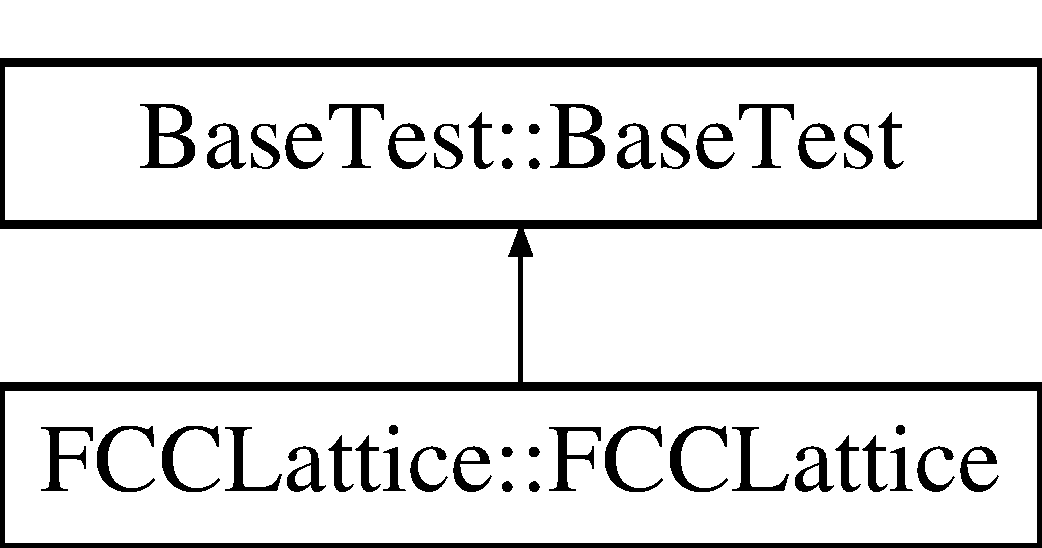
\includegraphics[height=2.000000cm]{classFCCLattice_1_1FCCLattice}
\end{center}
\end{figure}
\subsection*{Public Member Functions}
\begin{DoxyCompactItemize}
\item 
def \hyperlink{classFCCLattice_1_1FCCLattice_a80676c6dd31cab664be82fbdfead9576}{\_\-\_\-init\_\-\_\-}
\item 
def \hyperlink{classFCCLattice_1_1FCCLattice_a77866f6c592f0c8197833dcfd22e5145}{FCCEnergy}
\item 
def \hyperlink{classFCCLattice_1_1FCCLattice_a609b2ffb13217a24e05f12b1903eaaec}{TestResults}
\item 
def \hyperlink{classFCCLattice_1_1FCCLattice_aabdfdef0bb7ac45194ba57a22dff7ff8}{Verify}
\end{DoxyCompactItemize}


\subsection{Detailed Description}
\begin{DoxyVerb}FCCLattice test returns the optimal fcc lattice constant and energy per atom\end{DoxyVerb}
 

Definition at line 16 of file FCCLattice.py.



\subsection{Member Function Documentation}
\hypertarget{classFCCLattice_1_1FCCLattice_a80676c6dd31cab664be82fbdfead9576}{
\index{FCCLattice::FCCLattice@{FCCLattice::FCCLattice}!\_\-\_\-init\_\-\_\-@{\_\-\_\-init\_\-\_\-}}
\index{\_\-\_\-init\_\-\_\-@{\_\-\_\-init\_\-\_\-}!FCCLattice::FCCLattice@{FCCLattice::FCCLattice}}
\subsubsection[{\_\-\_\-init\_\-\_\-}]{\setlength{\rightskip}{0pt plus 5cm}def FCCLattice::FCCLattice::\_\-\_\-init\_\-\_\- (
\begin{DoxyParamCaption}
\item[{}]{ self, }
\item[{}]{ potentialname, }
\item[{}]{ element, }
\item[{}]{ TestDependencies = {\ttfamily \mbox{[}\mbox{]}}, }
\item[{}]{ args, }
\item[{}]{ kwargs}
\end{DoxyParamCaption}
)}}
\label{classFCCLattice_1_1FCCLattice_a80676c6dd31cab664be82fbdfead9576}
\begin{DoxyVerb}Pass the initialization arguments to the BaseTest initializer\end{DoxyVerb}
 

Definition at line 19 of file FCCLattice.py.

\hypertarget{classFCCLattice_1_1FCCLattice_a77866f6c592f0c8197833dcfd22e5145}{
\index{FCCLattice::FCCLattice@{FCCLattice::FCCLattice}!FCCEnergy@{FCCEnergy}}
\index{FCCEnergy@{FCCEnergy}!FCCLattice::FCCLattice@{FCCLattice::FCCLattice}}
\subsubsection[{FCCEnergy}]{\setlength{\rightskip}{0pt plus 5cm}def FCCLattice::FCCLattice::FCCEnergy (
\begin{DoxyParamCaption}
\item[{}]{ self, }
\item[{}]{ a}
\end{DoxyParamCaption}
)}}
\label{classFCCLattice_1_1FCCLattice_a77866f6c592f0c8197833dcfd22e5145}
\begin{DoxyVerb}This function computes the energy of the crystal formation given 
a certain lattice constant

It uses the ase helper function bulk to create a 1 atom periodic boundary
condition crystal with a specific structure\end{DoxyVerb}
 

Definition at line 24 of file FCCLattice.py.

\hypertarget{classFCCLattice_1_1FCCLattice_a609b2ffb13217a24e05f12b1903eaaec}{
\index{FCCLattice::FCCLattice@{FCCLattice::FCCLattice}!TestResults@{TestResults}}
\index{TestResults@{TestResults}!FCCLattice::FCCLattice@{FCCLattice::FCCLattice}}
\subsubsection[{TestResults}]{\setlength{\rightskip}{0pt plus 5cm}def FCCLattice::FCCLattice::TestResults (
\begin{DoxyParamCaption}
\item[{}]{ self}
\end{DoxyParamCaption}
)}}
\label{classFCCLattice_1_1FCCLattice_a609b2ffb13217a24e05f12b1903eaaec}
\begin{DoxyVerb}FCC Lattice Test Result

uses scipy fmin (a simplex method minimization tool), to find the optimal
lattice constant, and corresponding energy per atom\end{DoxyVerb}
 

Reimplemented from \hyperlink{classBaseTest_1_1BaseTest_ad7b3f3b61fcb07c94ae62cb12f060819}{BaseTest::BaseTest}.



Definition at line 39 of file FCCLattice.py.

\hypertarget{classFCCLattice_1_1FCCLattice_aabdfdef0bb7ac45194ba57a22dff7ff8}{
\index{FCCLattice::FCCLattice@{FCCLattice::FCCLattice}!Verify@{Verify}}
\index{Verify@{Verify}!FCCLattice::FCCLattice@{FCCLattice::FCCLattice}}
\subsubsection[{Verify}]{\setlength{\rightskip}{0pt plus 5cm}def FCCLattice::FCCLattice::Verify (
\begin{DoxyParamCaption}
\item[{}]{ self}
\end{DoxyParamCaption}
)}}
\label{classFCCLattice_1_1FCCLattice_aabdfdef0bb7ac45194ba57a22dff7ff8}
\begin{DoxyVerb}Simple verification script.  Creates a plot that shows the 
crystal energy in the neighborhood of the computed minimum, along
with the computed minimum, as a check \end{DoxyVerb}
 

Reimplemented from \hyperlink{classBaseTest_1_1BaseTest_a1857df472a65cef53372455376136409}{BaseTest::BaseTest}.



Definition at line 58 of file FCCLattice.py.



The documentation for this class was generated from the following file:\begin{DoxyCompactItemize}
\item 
tests/FCCLattice.py\end{DoxyCompactItemize}

\hypertarget{classNullTest_1_1NullTest}{
\section{NullTest::NullTest Class Reference}
\label{classNullTest_1_1NullTest}\index{NullTest::NullTest@{NullTest::NullTest}}
}
Inheritance diagram for NullTest::NullTest:\begin{figure}[H]
\begin{center}
\leavevmode
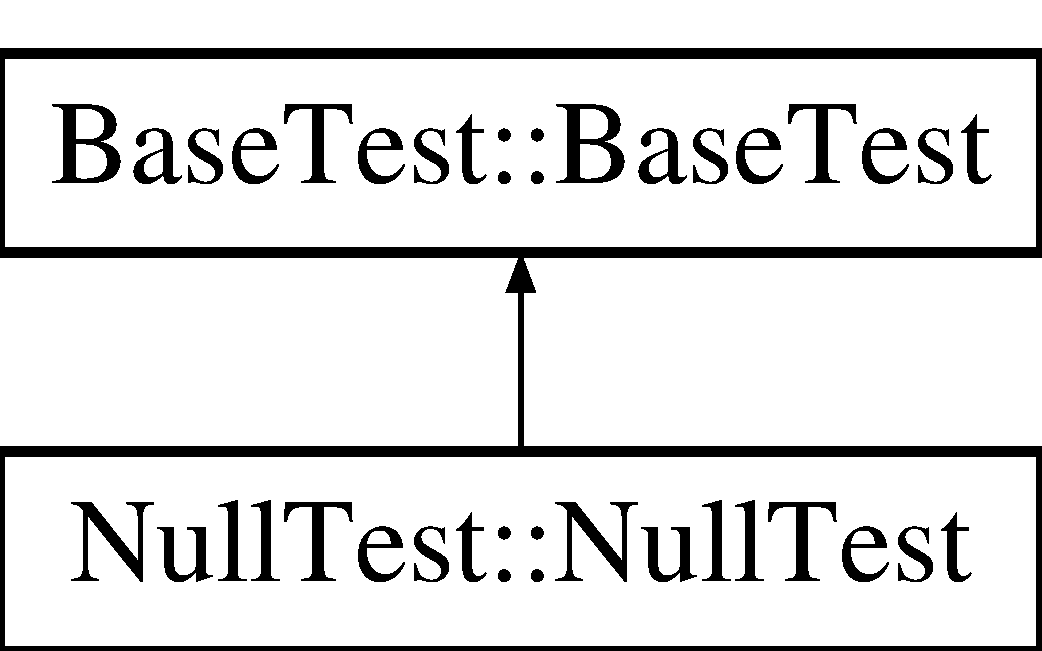
\includegraphics[height=2.000000cm]{classNullTest_1_1NullTest}
\end{center}
\end{figure}
\subsection*{Public Member Functions}
\begin{DoxyCompactItemize}
\item 
\hypertarget{classNullTest_1_1NullTest_ad0d8edee8b2eefb82e1bd0a5cc70baea}{
def {\bfseries \_\-\_\-init\_\-\_\-}}
\label{classNullTest_1_1NullTest_ad0d8edee8b2eefb82e1bd0a5cc70baea}

\item 
def \hyperlink{classNullTest_1_1NullTest_a7e6be14efc9b8191860c5d6bd62f0088}{TestResults}
\item 
def \hyperlink{classNullTest_1_1NullTest_a129b504762a05e76a355e6ef482ac8ab}{Verify}
\end{DoxyCompactItemize}


\subsection{Detailed Description}
\begin{DoxyVerb}NullTest does nothing, but serves as an example test.

    It inherits its functionality from BaseTest, and serves as a template for future
tests.  

Simply copy NullTest.py, and rename the file, and class name, and rewrite TestResults
\end{DoxyVerb}
 

Definition at line 11 of file NullTest.py.



\subsection{Member Function Documentation}
\hypertarget{classNullTest_1_1NullTest_a7e6be14efc9b8191860c5d6bd62f0088}{
\index{NullTest::NullTest@{NullTest::NullTest}!TestResults@{TestResults}}
\index{TestResults@{TestResults}!NullTest::NullTest@{NullTest::NullTest}}
\subsubsection[{TestResults}]{\setlength{\rightskip}{0pt plus 5cm}def NullTest::NullTest::TestResults (
\begin{DoxyParamCaption}
\item[{}]{ self}
\end{DoxyParamCaption}
)}}
\label{classNullTest_1_1NullTest_a7e6be14efc9b8191860c5d6bd62f0088}
\begin{DoxyVerb}Required module, the TestResults Module returns a dictionary of result. 

of the form { 'NameOfValue' : value, 'NameOfSecondValue' : secondvalue }

This is where your test code goes.  Feel free to write other methods if necessary.
\end{DoxyVerb}
 

Reimplemented from \hyperlink{classBaseTest_1_1BaseTest_ad7b3f3b61fcb07c94ae62cb12f060819}{BaseTest::BaseTest}.



Definition at line 25 of file NullTest.py.

\hypertarget{classNullTest_1_1NullTest_a129b504762a05e76a355e6ef482ac8ab}{
\index{NullTest::NullTest@{NullTest::NullTest}!Verify@{Verify}}
\index{Verify@{Verify}!NullTest::NullTest@{NullTest::NullTest}}
\subsubsection[{Verify}]{\setlength{\rightskip}{0pt plus 5cm}def NullTest::NullTest::Verify (
\begin{DoxyParamCaption}
\item[{}]{ self}
\end{DoxyParamCaption}
)}}
\label{classNullTest_1_1NullTest_a129b504762a05e76a355e6ef482ac8ab}
\begin{DoxyVerb}Optional verify script to be used to generate a visual output for

quick check that everything is going alright\end{DoxyVerb}
 

Reimplemented from \hyperlink{classBaseTest_1_1BaseTest_a1857df472a65cef53372455376136409}{BaseTest::BaseTest}.



Definition at line 36 of file NullTest.py.



The documentation for this class was generated from the following file:\begin{DoxyCompactItemize}
\item 
tests/NullTest.py\end{DoxyCompactItemize}

\printindex
\end{document}
